%=====================================================================
% 3  Feynman 演算（后半：3.7--3.14  非线性方程、树的计数与有效作用量）
% 原文：Section 3.7--3.14. Nonlinear equations and trees / The case d=1 /
%       Counting trees and Cayley's theorem / Counting trees with conditions /
%       Counting oriented trees / The matrix-tree theorem /
%       1-particle irreducible diagrams and the effective action /
%       1-particle irreducible diagrams and the Legendre transform
%       （arXiv:2409.03117v1, p. 40--50）
% 说明：本文件为第 3 章后半，接 sec03a-feynman.tex，故不另起 \section。
%=====================================================================

\begin{keytakeaways}
\begin{itemize}
  \item \textbf{物理图像：} 临界点处的作用量取值（即树的贡献之和）可以完全按树来组织：把临界点方程改写成压缩映射的不动点方程并反复代入，展开的每一项对应一棵树，且因树的顶点数比边数恰好多一，两项贡献之差使每棵树恰好被计入一次。这就是“树定理”的组合内容，也是全章 Feynman 演算的组合骨架。
  \item \textbf{数学工具：} 环路围道积分加变量代换与留数（等价于 Lagrange--B\"urmann 反演）提取 Taylor 系数；Kirchhoff 多项式与图的 Laplace 算子；以及“删去全部桥”把连通图唯一地收缩为以 1PI 子图为顶点的骨架树。
  \item \textbf{关键结论：} Cayley 定理（带标号树共 $n^{n-2}$ 棵）、带颜色与带条件（三价、有向）的树计数、加权矩阵树定理；有效作用量按单粒子不可约（1PI）图展开，其经典（树）部分等于原作用量临界值取负，并与生成函数的对数由 Legendre 变换互相确定。
  \item \textbf{易错点：} 三价树推论中的顶点数指标、矩阵树定理里邻接矩阵与 Laplace 算子的符号约定及前置因子、有效作用量展开中每圈对应的 $\hbar$ 幂次，以及 Legendre 变换的符号与变量选择，都须回原文逐项核对。
\end{itemize}
\end{keytakeaways}

\bigskip
\noindent\rule{\textwidth}{0.6pt}
\bigskip

\subsection{非线性方程与树}\label{treepar}

正如我们已经注意到的，定理 \ref{trees1l} 不涉及积分，是纯组合性的。因此，该定理应当存在一个纯组合的证明。这样的证明确实存在。这里我们将对定理的第一个论断（公式 (\ref{treeeq})）给出一个组合证明。

考虑用来定义临界点 $x_0$ 的方程 $S'(x)=0$。该方程可以写成 $x=\beta(x)$，其中
$$
\beta(x):=\sum_{i\ge 1}g_i\frac{B^{-1}B_i(x, \ldots ,x,-)}{(i-1)!},
$$
这里 $B^{-1}: V^*\to V$ 是相应于形式 $B^{-1}$ 的算子。

在幂级数范数的意义下，$\beta$ 是压缩映射。于是对任意初始向量（例如 $0\in V$），有 $x_0=\lim_{N\to \infty}\beta^N(x)$。换句话说，只要不断把级数 $\beta(x)$ 代入其自身，就能得到 $x_0$。这导致对树的求和（试解释其缘由！）。更确切地说，我们得到 $x_0$ 的如下表达式：
$$
x_0=\sum_{\bold n}\prod_i g_i^{n_i}\sum_{\Gamma\in G^{(0)}(\bold n,1)}
\frac{\Bbb F_\Gamma}{|{\rm Aut}(\Gamma)|},
$$
其中 $G^{(0)}(\bold n,1)$ 是带一个外顶点、且有 $n_i$ 个 $i$ 价内顶点的树的集合。

现在，由于 $S(x)=\frac{B(x,x)}{2}-\sum_i g_i\frac{B_i(x, \ldots ,x)}{i!}$，表达式 $-S(x_0)$ 等于诸表达式 $\prod_i g_i^{n_i}\frac{\Bbb F_\Gamma}{|{\rm Aut}(\Gamma)|}$ 对一切（不含外顶点的）树的求和。确实，项 $\frac{B(x_0,x_0)}{2}$ 对应于把两棵带外顶点的树粘合起来（将两个外顶点等同，使它们消失）；因此它对应于对带标记边的树求和，亦即每棵树被计入的次数等于其边数。另一方面，项 $g_i\frac{B_i(x_0, \ldots ,x_0)}{i!}$ 对应于把 $i$ 棵带外顶点的树在这些顶点处粘合在一起（得到带标记顶点的树）。因此 $\sum_i g_i\frac{B_i(x_0, \ldots ,x_0)}{i!}$ 对应于对带标记顶点的树求和，亦即每棵树被计入的次数等于其顶点数。但树的顶点数比边数多 $1$。于是，上述两个贡献之差 $-S(x_0)$ 对应于对树的求和，且每棵树恰好被计入一次。这就蕴含公式 (\ref{treeeq})。

% [Tutor Note: 这段双重计数是全节的枢纽，原文用一句“explain why!”把它留作练习。补足如下：代入迭代之所以给出树，是因为 β 以 $g_i$ 为形式小参数（按 $g$ 的幂次）是压缩映射：每次代入都在原有结构的某个“外顶点”处长出一个新的内顶点，于是逐次迭代给出按顶点数递增的树展开，并在形式幂级数意义下收敛；而因子 1/|Aut(Γ)| 来自把外顶点标记为可区别后除以自同构群。符号的来历则是 |V|-|E|=1（连接图的欧拉示性数），这正是“顶点标记计数减边标记计数等于每棵树计一次”的来源。]

\subsection{$d=1$ 的情形}

在 $d=1$ 的情形，树和 $-S(x_0)$ 可以更显式地算出。即设
$$
S(x):=\frac{x^2}{2}-gh(x)
$$
其中 $h(x)=\sum_{n\ge 0}c_nx^n$，$c_1\ne 0$。则 $x_0$ 是方程 $x=gh'(x)$ 的解，亦即 $x_0=f(g)$，其中 $x=f(y)$ 是 $y=\frac{x}{h'(x)}$ 的反函数。于是树近似取如下形式：$-S(x_0)=F(g)$，其中
$$
F(g)=-\frac{f(g)^2}{2}+gh(f(g)). 
$$
因此
$$
F'(g)=-f(g)f'(g)+h(f(g))+gh'(f(g))f'(g).
$$
但 $h'(f(g))=\frac{f(g)}{g}$，故第一项与第三项相消，得到
$$
F'(g)=h(f(g)), 
$$
从而
\begin{equation}\label{deq1}
-S(x_0)=\int_0^g h(f(a))da.
\end{equation}

\subsection{树的计数与 Cayley 定理}

本节我们将把定理 \ref{trees1l} 应用于树的计数问题，特别地证明 Cayley 的一个经典定理：带 $n$ 个顶点的带标号树的数目为 $n^{n-2}$。

我们考虑的情形与上文例 \ref{treeexa} 中所考虑的基本相同：$d=1$，$B_i=1$，$g_i=g$。于是 $S(x)=\frac{x^2}{2}-ge^x$。由定理 \ref{trees1l}，有
$$
\sum_{n\ge 0}g^n\sum_{\Gamma \in T(n)}\frac{1}{|{\rm Aut}(\Gamma)|}=
-S(x_0),
$$
其中 $T(n)$ 是带 $n$ 个顶点的树的同构类的集合，而 $x_0$ 是方程 $S'(x)=0$ 的根，即 $x=ge^x$。

换句话说，设 $x=f(y)$ 是 $y=xe^{-x}$ 在 $x=0$ 附近的反函数，则 $x_0=f(g)$。函数 $f(y)$ 与（主支的）\emph{Lambert 函数} $W(y)$ 由公式 $f(y)=-W(-y)$ 相联系。由 \eqref{deq1} 得
$$
-S(x_0)=\int_0^g e^{f(a)}da=\int_0^g\frac{f(a)}{a}da.
$$
因此只需再求 $f$ 的 Taylor 展开。该展开由下述经典结果给出。

\begin{proposition}
有
$$
f(g)=\sum_{n\ge 1}\frac{n^{n-2}}{(n-1)!}g^n.
$$
\end{proposition}

\begin{proof}
令 $f(g)=\sum_{n\ge 1}a_ng^n$。则
$$
a_n=\frac{1}{2\pi i}\oint\frac{f(g)}{g^{n+1}}dg=
\frac{1}{2\pi i}\oint\frac{x}{(xe^{-x})^{n+1}}d(xe^{-x})=
$$
$$
\frac{1}{2\pi i}\oint e^{nx}\frac{1-x}{x^n}dx=
\frac{n^{n-1}}{(n-1)!}-\frac{n^{n-2}}{(n-2)!}=
\frac{n^{n-2}}{(n-1)!}.
$$
\end{proof}

% [Tutor Note: 证明中的围道积分只绕 g=0（或等价地 x=0）取留数。代换 g=xe^{-x} 给出 dg=(1-x)e^{-x}dx，于是被积式化为 e^{nx}(1-x)/x^n dx，两个留数分别是 e^{nx}/x^n 与 e^{nx}/x^{n-1} 在 x=0 处的系数，即 n^{n-1}/(n-1)! 与 n^{n-2}/(n-2)!。这实际上是 Lagrange--Bürmann 反演公式的特例：若 g=x/φ(x)，则 [g^n]f(g)=n^{-1}[x^{n-1}]φ(x)^n，此处 φ=e^{x}。另需注意 f 只在 g=0 附近取主支（即 Lambert W 的主支），g 增大到 1/e 处两支相交，级数收敛半径正是 1/e。]

于是得到
$$
-S(x_0)=\int_0^g\frac{f(a)}{a}da=\sum_{n\ge 1}\frac{n^{n-2}}{n!}g^n.
$$
这表明
$$
\sum_{\Gamma\in T(n)}\frac{1}{|{\rm Aut}(\Gamma)|}=\frac{n^{n-2}}{n!}.
$$
但带 $n$ 个顶点的无标号树的每个同构类都有 $\frac{n!}{|{\rm Aut}(\Gamma)|}$ 个不同的标号方式。因此我们得到

\begin{corollary} (A. Cayley) 带 $n$ 个顶点的带标号树的数目为 $n^{n-2}$。
\end{corollary}

\subsection{带条件的树计数}

类似地，我们可以计数对顶点加了条件的带标号树。例如，我们计算带 $m$ 个顶点的带标号三价树的数目（即只含 1 价与 3 价顶点的树）。显然 $m=2k$，否则不存在这样的树。相应的作用量泛函为
$$
S(x)=\tfrac{x^2}{2}-g(x+\tfrac{x^3}{6}).
$$
于是临界点 $x_0$ 由方程
$$
x=g(1+\tfrac{x^2}{2}),
$$
给出，从而
$$
x_0=\frac{1-\sqrt{1-2g^2}}{g}.
$$
因此由 \eqref{deq1}，树和等于
$$
-S(x_0)=\int_0^g\left(\tfrac{1-\sqrt{1-2a^2}}{a}+\tfrac{(1-\sqrt{1-2a^2})^3}{6a^3}\right)da=
$$
$$
\frac{2}{3}\int_0^g\tfrac{1-(1+a^2)\sqrt{1-2a^2}}{a^3}da=
\frac{(1-2g^2)^{\frac{3}{2}}-(1-3g^2)}{3g^2}.
$$
将其展成 Taylor 级数，可得
$$
-S(x_0)=\sum_{n=1}^\infty \frac{1\cdot 3\cdot \, \cdots \,\cdot
  (2n-3)}{(n+1)!}g^{2n}.
$$
于是得到

\begin{corollary}
带 $2n$ 个顶点的三价带标号树的数目 $N_k$ 为 $(2k-3)!!\frac{(2k)!}{(k+1)!}$。
\end{corollary}

% [Tutor Note: 此处原文指标确有笔误：推论说“带 2n 个顶点”，但上下文（m=2k、$N_k$、以及括号内的 (2k-3)!! 与 (2k)!）都表明应为“带 2k 个顶点”，n 是前一节 Cayley 计数留下的指标。建议按 2k 读。可用小值核对：k=2 时 (1)!!·4!/3!=4，与正文“单个树、4! 个标号模 6 阶群”的 N_2=4 相符；k=3 时 3!!·6!/4!=3·30=90，与正文的 N_3=90 相符。]

例如，$N_1=1$（单条边），$N_2=4$（单棵树，$4!$ 个标号模去一个 $6$ 阶群），$N_3=90$（单棵树，$6!$ 个标号模去一个 $8$ 阶群），等等。

\begin{figure}[htbp]
  \centering
  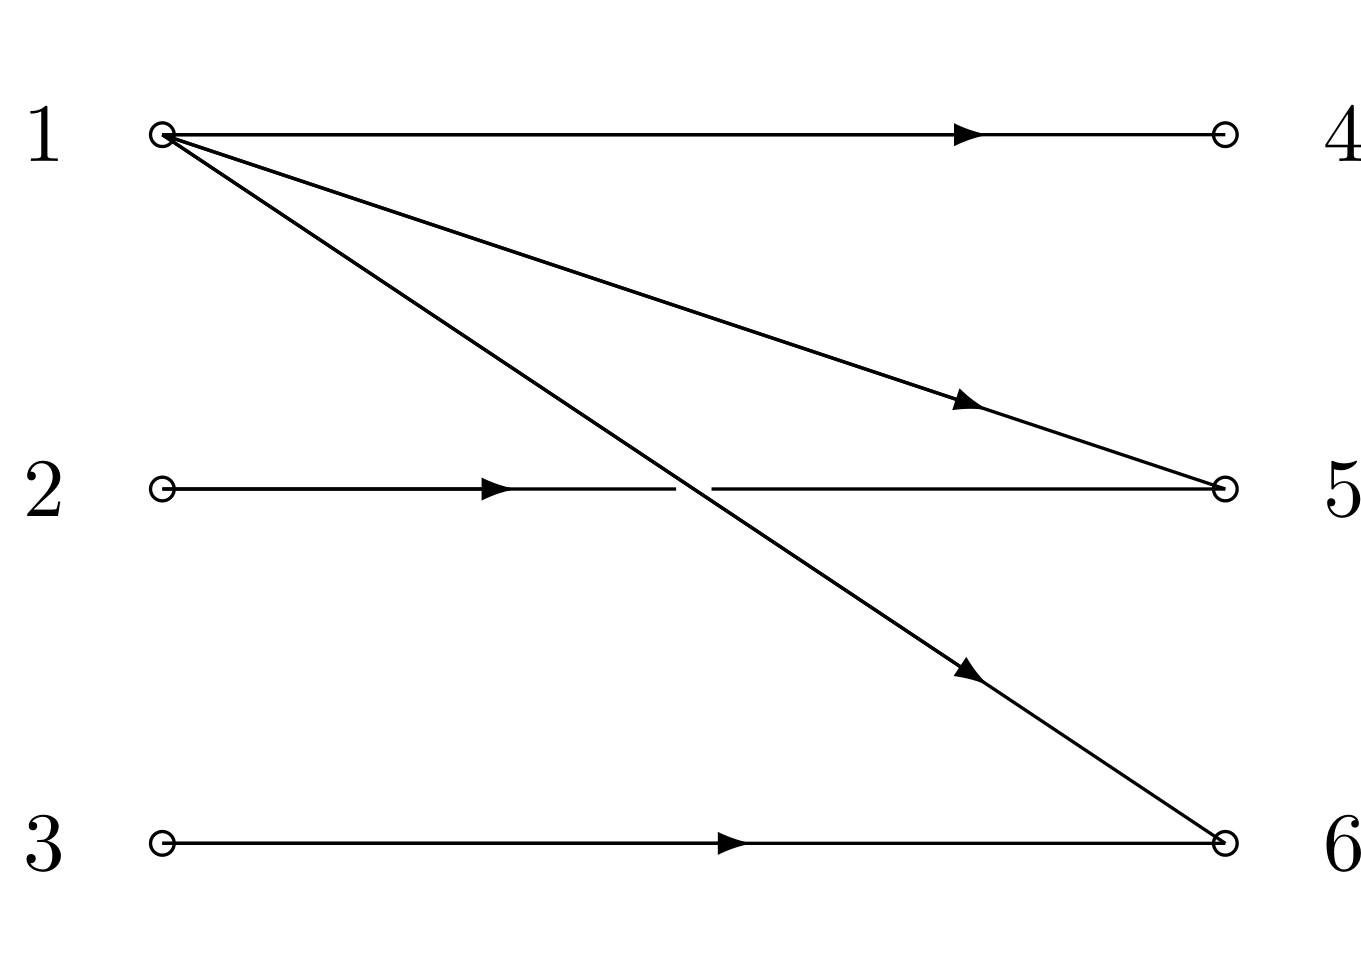
\includegraphics[width=5.76cm]{figures/fig-07.png}
  \caption{一个含 3 个源点与 3 个汇点的带标号有向树。\figorig{43}{7}}
  \label{fig:7}
\end{figure}

\subsection{有向树的计数}

Feynman 演算不仅可以用来计数无向图，也可以用来计数有向图。例如，假设我们要计数带标号的有向树，其顶点或为源点、或为汇点（见图 \ref{fig:7}）。此时容易看出（试检验之！），相应的积分问题是二维的，作用量为 $S=xy-be^x-ae^y$（形式 $xy$ 不是正定的，但这无关紧要，因为我们的计算是纯粹形式的）。于是临界点由方程
$$
xe^{-y}=a,\ ye^{-x}=b.
$$
求出。与前面一样，以下述形式寻找解 $(x,y)=(x_0,y_0)$：
$$
x=a+\sum_{p\ge 1,q\ge 1} c_{pq}a^pb^q,\ y=b+\sum_{p\ge 1,q\ge 1} d_{pq}a^pb^q.
$$
与无向树情形类似的计算（用留数）给出
$$
c_{pq}=\frac{1}{(2\pi i)^2}\oint\oint\frac{x}{a^{p+1}b^{q+1}}da\wedge db=
$$
$$
\frac{1}{(2\pi i)^2}\oint\oint \frac{e^{qx+py}}{x^py^{q+1}}(1-xy)dx\wedge dy=
\frac{q^{p-1}p^{q-1}}{(p-1)!q!}.
$$
类似地，$d_{pq}=\frac{q^{p-1}p^{q-1}}{p!(q-1)!}$。现在，与无向情形类似，可得 $-a\partial_aS(x,y)=x$，$-b\partial_bS(x,y)=y$，故
$$
-S(x,y)=b+\int_0^a\frac{x}{u}du=
a+b+\sum_{p,q\ge 1}\frac{p^{q-1}q^{p-1}}{p!q!}a^pb^q
$$
这表明带 $p$ 个源点与 $q$ 个汇点的带标号树的数目为 $p^{q-1}q^{p-1}\frac{(p+q)!}{p!q!}$。特别地，若指定哪些顶点为源点、哪些为汇点，则带标号树的数目为 $p^{q-1}q^{p-1}$。

\begin{exercise} 请详细完成这一计算。
\end{exercise}

\subsection{矩阵树定理}

这些计算可以推广，用以计算\emph{着色}带标号树的数目。为此，首先需要定义\emph{Kirchhoff 多项式} $K_m(\bold u)$。即：对一组变量 $\bold u:=(u_{ik})$，$1\le i\ne k\le m$，$u_{ik}=u_{ki}$，考虑二次型
$$
U(\bold y):=\sum_{1\le i<k\le m}u_{ik}(y_i-y_k)^2.
$$
一般地，它有由 $\bold 1=(1,...,1)$ 张成的一维核，因而在由方程 $\sum_i y_i=0$ 定义的子空间上非退化。该子空间带有一个体积形式 $\omega_0(v_1,...,v_{m-1}):=\omega(v_1,...,v_{m-1},\bold 1)$，其中 $\omega$ 是 $\Bbb R^m$ 上的标准体积形式；关于此形式有
$$
K_m(\bold u):=\det U=\det(\delta_{i\ell}\sum_{k\ne \ell} u_{k\ell }-u_{i\ell})_{(j)}
$$
对任意 $1\le j\le m$ 成立，其中下标 $(j)$ 表示删去第 $j$ 行与第 $j$ 列。多项式 $K_m$ 称为\emph{Kirchhoff 多项式}。例如 $K_2=u_{12}$，$K_3=u_{12}u_{13}+u_{13}u_{23}+u_{12}u_{23}$，等等。

现设 $\bold p=(p_1,...,p_m)$ 为正整数的 $m$ 元组，$\bold r=(r_{ij},1\le i\le j\le m)$ 为一组非负整数，满足 $|\bold r|=|\bold p|-1$，其中 $|\bold r|:=\sum_{i\le j}r_{ij}$，$|\bold p|:=\sum_k p_k$。设树的顶点被赋予颜色 $1,...,m$，而我们想计算带标号树的数目 $N(\bold p,\bold r)$：前 $p_1$ 个顶点染颜色 $1$，接下来的 $p_2$ 个染颜色 $2$，……，最后的 $p_m$ 个染颜色 $m$，且有 $r_{ij}$ 条边连接颜色 $i$ 的顶点与颜色 $j$ 的顶点。

只需计算多项式
$$
Q_{\bold p}(\bold z):=\sum_{\bold r: |\bold r|=|\bold p|-1} N(\bold p,\bold r)\prod_{i\le j}z_{ij}^{r_{ij}}. 
$$
\begin{theorem}\label{mt} 有
$$
Q_\bold p(\bold z)=
(p_1...p_m)^{-1}K(p_kz_{k\ell}p_\ell, k\ne \ell)\prod_\ell(\sum_k p_kz_{k\ell})^{p_\ell-1}.
$$
\end{theorem}

注意，当 $m=1$、$\bold z=1$ 时这恢复 Cayley 定理；而当 $m=2$、$\bold z=\begin{pmatrix} 0& 1\\ 1& 0\end{pmatrix}$ 时，它恢复我们对有向树的计数。

\begin{proof}
我们给每种颜色 $j$ 配一个实变量 $x_j$。则相应的作用量为
$$
S(x,y)=\frac{1}{2}x^TB x-\sum_{j=1}^m a_je^{x_j},
$$
其中 $B=(b_{ij})$ 是矩阵 $\bold z:=(z_{ij})$（$z_{ij}=z_{ji}$）的逆。于是由定理 \ref{trees1l}，$Q_{\bold p}(\bold z)$ 是 $-S(x)$ 中 $\prod_k a_k^{p_k}$ 的系数，其中 $x$ 是 $S$ 的临界点。

$S$ 的临界点方程为
$$
\sum_i x_ib_{ij}e^{-x_j}=a_j.
$$
令 $X_j:=\sum_i x_ib_{ij}$，则 $x_i=\sum_jz_{ij}X_j$，$a_i=X_ie^{-x_i}$，且对一切 $j$ 有
$$
-S(x)=\int X_j\frac{da_j}{a_j}
$$
换句话说，$-S(x)$ 中 $\prod_k a_k^{p_k}$ 的系数等于 $X_j(\bold z,\bold a)$ 中同一单项式的系数除以 $p_j$。因此，以 $D_T(\bold z)$ 记 $\bold z$ 对应于子集 $T\subset \lbrace 1,...,m\rbrace$ 的主子式，得到
$$
Q_{\bold p}(\bold z)=\tfrac{p_j^{-1}}{(2\pi i)^m}\oint X_j(\prod_k a_k^{-p_k-1})d\bold a=
$$
$$
\tfrac{p_j^{-1}}{(2\pi i)^m}\oint X_j(\prod_k (X_ke^{-x_k})^{-p_k-1})d(X_1e^{-x_1})\wedge...\wedge d(X_me^{-x_m})=
$$
$$
\tfrac{p_j^{-1}}{(2\pi i)^m}\oint \sum_{T\subset \lbrace 1,...,m\rbrace}(-1)^{|T|}D_T(\bold z)X_j(\prod_{\ell\notin T}X_\ell^{-1})(\prod_\ell X_\ell^{-p_\ell})e^{\sum_{k,\ell} p_kz_{k\ell}X_\ell}dX_1\wedge...\wedge dX_m
$$
$$
=p_j^{-1}\sum_{T\subset \lbrace 1,...,m\rbrace}(-1)^{|T|}\frac{p_j-1+\delta_{jT^c}}{\sum_k p_kz_{kj}}D_T(\bold z)\prod_\ell\frac{(\sum_k p_kz_{k\ell})^{p_\ell-\delta_{\ell T}}}{(p_\ell-\delta_{\ell T})!}=
$$
\scriptsize
$$
p_j^{-1}
\left(\frac{p_j-1}{\sum_k p_kz_{kj}}\det(\delta_{i\ell}\sum_k p_kz_{k\ell}-z_{i\ell}p_\ell)+
\det(\delta_{i\ell}\sum_k p_kz_{k\ell}-z_{i\ell}p_\ell)_{(j)}\right)\prod_\ell\frac{(\sum_k p_kz_{k\ell})^{p_\ell-1}}{p_\ell!},
$$
\normalsize
其中当 $\ell\in T$ 时 $\delta_{\ell T}=1$，否则为 $0$。第一个行列式为零，故得到
$$
Q_{\bold p}(\bold z)=(p_1...p_m)^{-1}\det(\delta_{i\ell}\sum_k p_kz_{k\ell}p_\ell-p_iz_{i\ell}p_\ell)_{(j)}\prod_\ell\frac{(\sum_k p_kz_{k\ell})^{p_\ell-1}}{p_\ell!}.
$$
这就蕴含定理。
\end{proof}

% [Tutor Note: “第一个行列式为零”这一步原文省略了理由：矩阵 M_{iℓ}=δ_{iℓ}·Σ_k p_k z_{kℓ} − z_{iℓ}p_ℓ 的第 i 行之和为 Σ_ℓ M_{iℓ}=Σ_k p_k z_{ki} − Σ_ℓ z_{iℓ}p_ℓ，而 z 对称（z_{iℓ}=z_{ℓi}）使两项相等，故每行之和为 0，det M=0。剩下的那个主子式正是加权矩阵树定理的“加权度−加权邻接”矩阵。另注意此处图论约定：z 是邻接矩阵的对称化（无自环，z_{ii} 不出现），Δ_Γ=D_Γ−A_Γ 取的是通常的（非负）Laplace 矩阵，故 U 半正定、核为一维常数向量；推论中的 1/m 因子正是来自“λ 中有一个零本征值”，即对 m−1 个非零本征值取积再除以 m。]

定理 \ref{mt} 是\emph{Kirchhoff 矩阵树定理}的加权版本，后者是 Cayley 定理的推广。更确切地说，取 $\bold z=A_\Gamma$ 为图 $\Gamma$（无自环）的邻接矩阵，$m$ 为 $\Gamma$ 的顶点数，并对一切 $i$ 取 $p_i=1$。则 $Q_{\bold p}(\bold z)=N_\Gamma$ 是 $\Gamma$ 的生成树的数目，而定理 \ref{mt} 断言
$$
N_\Gamma=\det U,
$$
其中 $U$ 是二次型
$$
U(\bold y)=\sum_{i<j}(A_\Gamma)_{ij}(y_i-y_j)^2=(\Delta_\Gamma \bold y,\bold y),
$$
其中 $\Delta_\Gamma=D_\Gamma-A_\Gamma$ 是 $\Gamma$ 的 Laplace 算子（$D_\Gamma$ 为顶点度数的对角矩阵）。于是得到

\begin{corollary} (矩阵树定理)
$$
N_\Gamma=\frac{1}{m}\lambda_1...\lambda_{m-1},
$$
其中 $\lambda_i$ 是 $\Delta_\Gamma$ 的非零本征值。
\end{corollary}

当 $\Gamma$ 是完全图时，由这一结果得到 Cayley 定理：此时对一切 $i$ 有 $\lambda_i=m$，故 $N_\Gamma=m^{m-2}$。

\subsection{单粒子不可约图与有效作用量}

设 $Z=Z_S$ 是对应于作用量 $S$ 的配分函数。在前几个小节中我们已经看到，量 $\hbar\log\frac{Z_S}{Z_0}$ 的“经典”（或“树”）部分 $(\log\frac{Z_S}{Z_0})_0$ 是相当初等的计算——它就是作用量 $S(x)$ 的临界值取负号。因此，若能找到一个新“有效”作用量 $S_{\rm eff}$（$S$ 的一个“形变”），使得
$$
\hbar^{-1}(\log\tfrac{Z_{\rm S_{\rm eff}}}{Z_0})_0=\log\tfrac{Z_S}{Z_0}
$$
（即有效作用量的经典答案就是原作用量的量子答案），则作用量 $S$ 的量子理论便可视为已解出。换句话说，求解附属于 $S$ 的量子理论（即求出相应的积分）的问题，本质上归结为计算有效作用量 $S_{\rm eff}$ 的问题。

下面我们给出用 Feynman 图振幅计算有效作用量的方法，并将看到它在计算上比求连通图之和更容易。

\begin{definition}
设 $e$ 是连通图 $\Gamma$ 的一条边。若图 $\Gamma\setminus\ e$ 不连通，则称该边为\emph{桥}。不含桥的连通图称为\emph{单粒子不可约}（1PI）的。\footnote{这是物理术语；数学术语为“2-连通”。}
\end{definition}

为计算有效作用量，我们需要考虑带外线的图（但至少含一个内顶点）。这样的图 $\Gamma$（带 $N$ 条外线）称为单粒子不可约的，如果相应的“截肢”图（即从 $\Gamma$ 中删去外线所得的图）是单粒子不可约的。特别地，含一个内顶点的图总是单粒子不可约的；而无内顶点的单边图则\emph{不}定义为单粒子不可约。桥与单粒子不可约图的概念见图 \ref{fig:8}。

\begin{figure}[htbp]
  \centering
  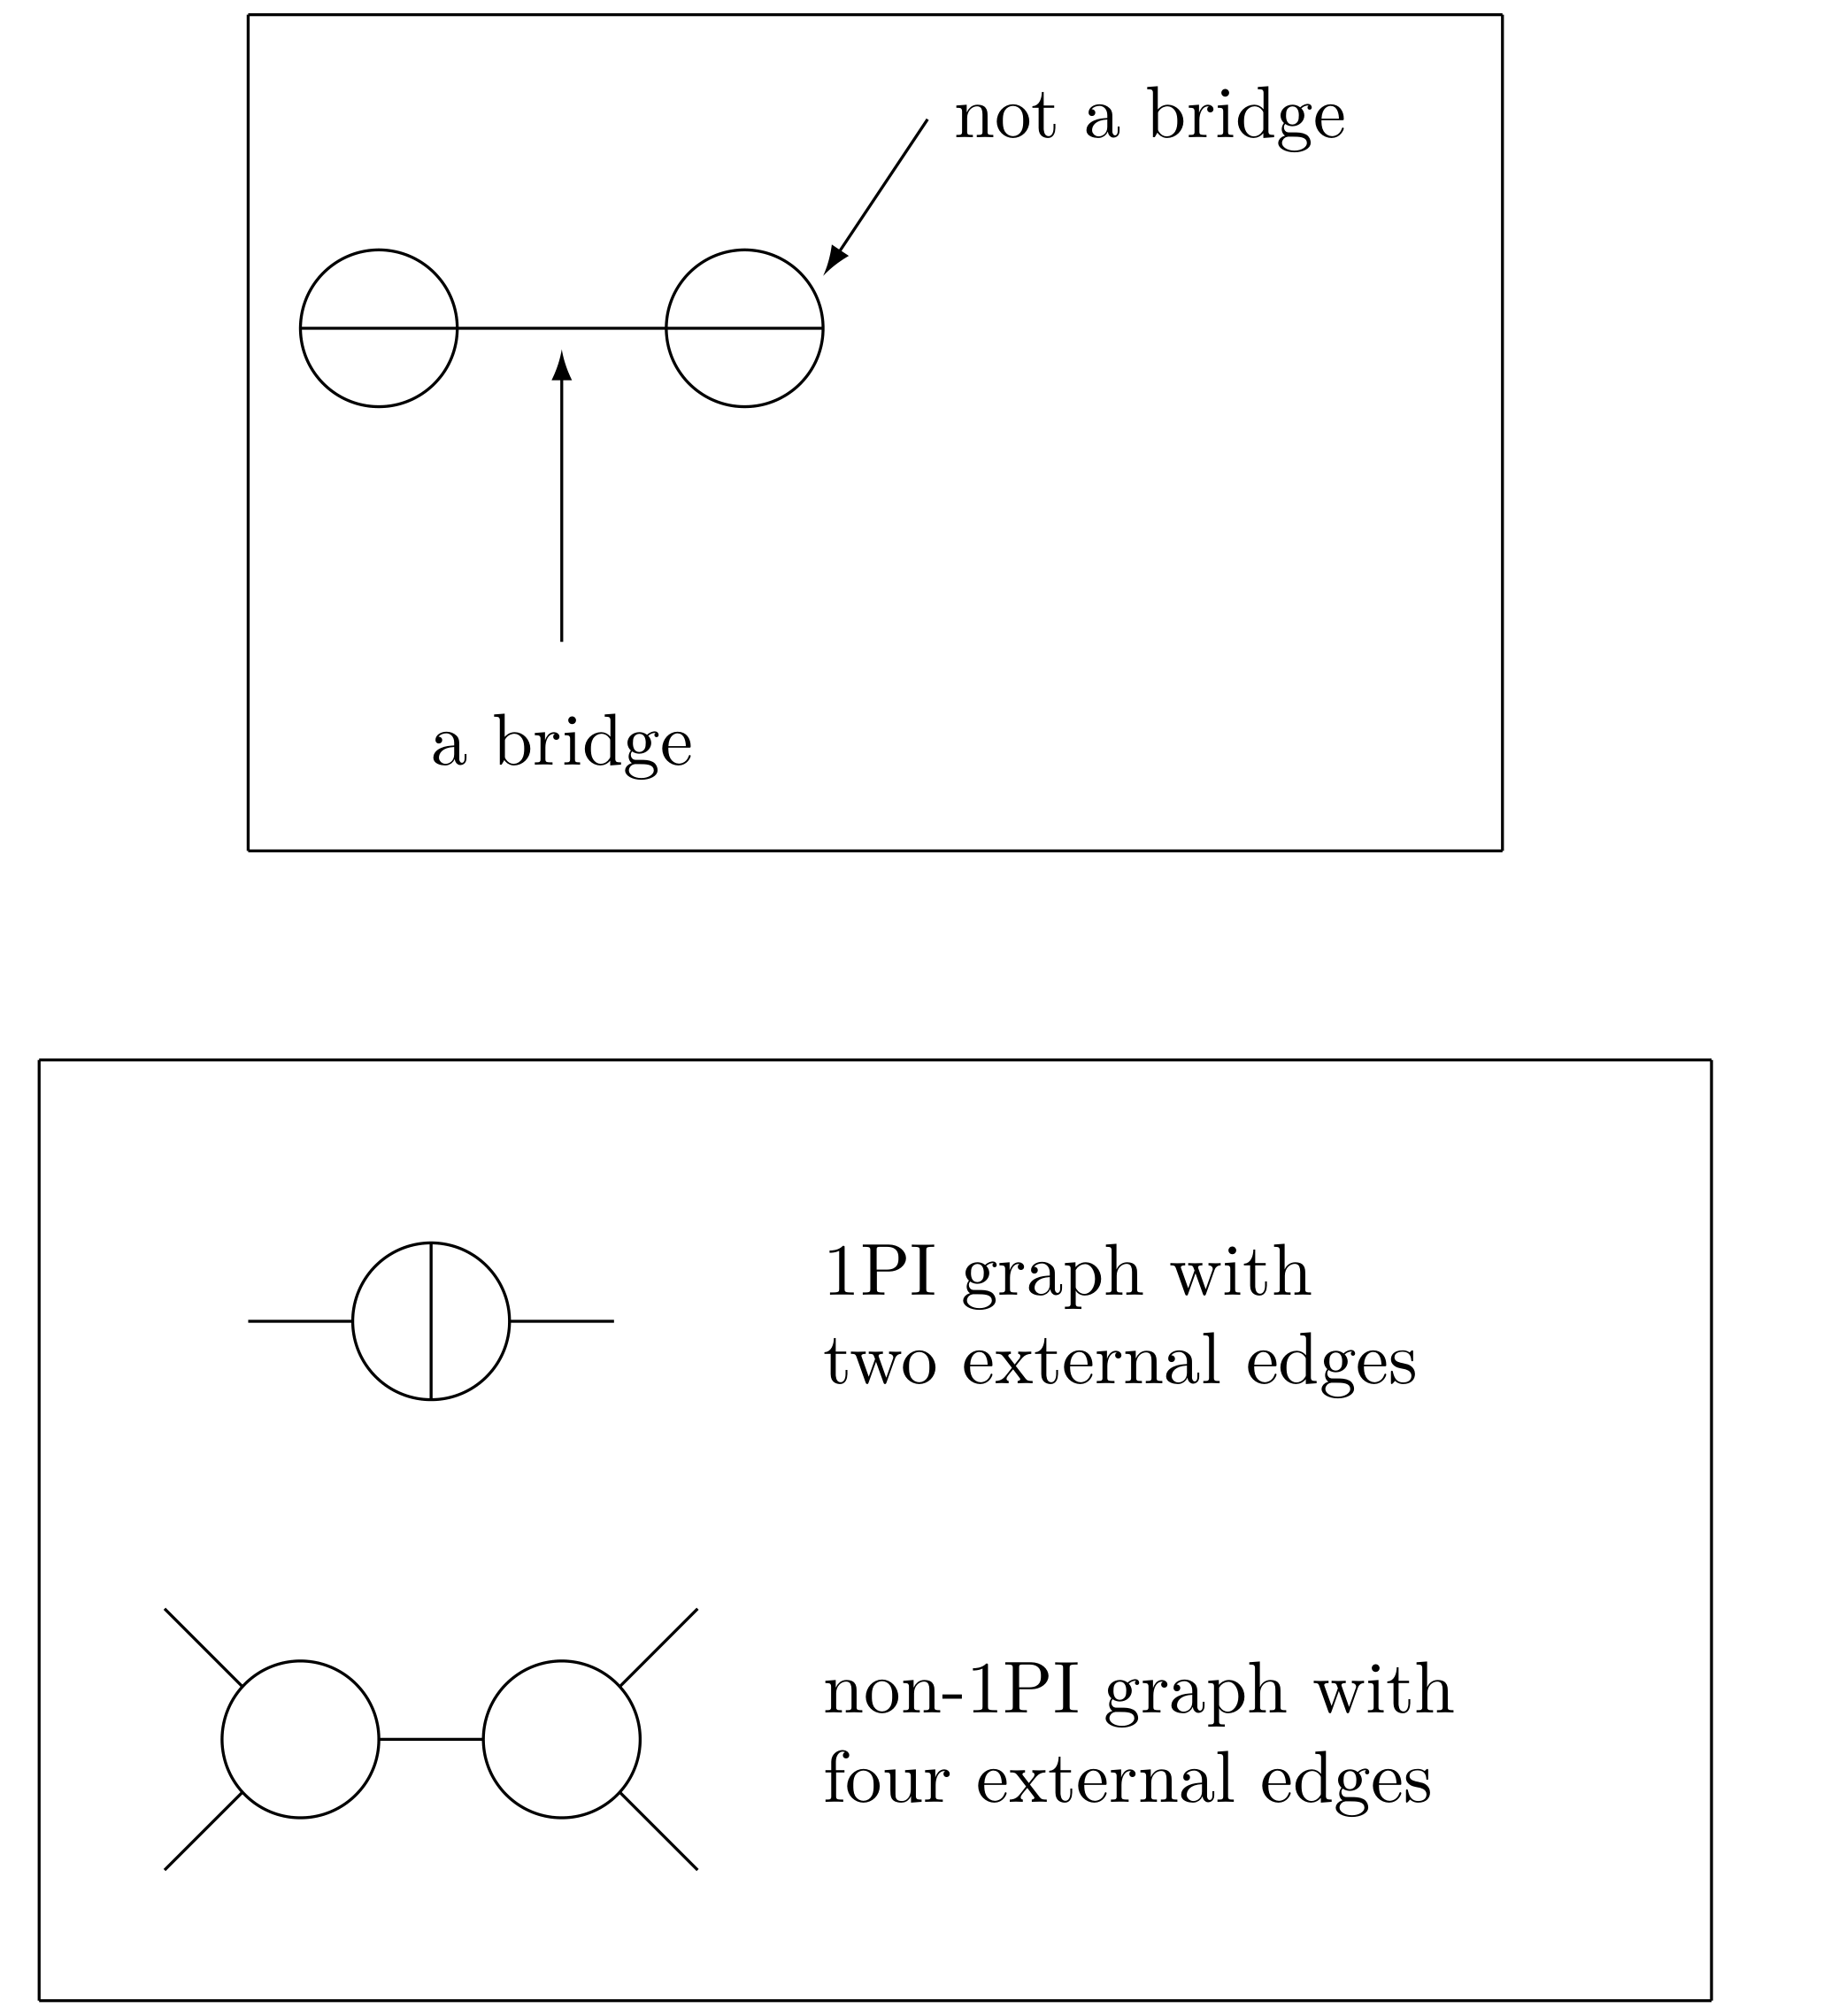
\includegraphics[width=8.76cm]{figures/fig-08.png}
  \caption{（原文无图题）\figorig{47}{8}}
  \label{fig:8}
\end{figure}

用 $G_{\rm 1PI}(\bold n,N)$ 表示如下单粒子不可约图的同构类的集合：它们有 $N$ 条外线，且对每个 $i$ 有 $n_i$ 个 $i$ 价内顶点（这里同构不允许移动外线）。

\begin{theorem} \label{effac}
有效作用量 $S_{\rm eff}$ 由公式
$$
S_{\rm eff}(x)=
 \frac{B(x,x)}{2}-
\sum_{i\ge 0}\frac{{\mathcal B}_i(x,...,x)}{i!},
$$
给出，其中
$$
{\mathcal B}_N(x, \ldots ,x)=\hbar\sum_{\bold n}\prod_i (g_i\hbar^{\frac{i}{2}-1})^{n_i}
\sum_{\Gamma\in G_{\rm 1PI}(\bold
  n,N)}\frac{\Bbb F_\Gamma(Bx, \ldots ,Bx)}{|{\rm Aut}(\Gamma)|}.
$$
\end{theorem}

% [Tutor Note: 这里的 ℏ 幂次是“圈数记账”，最易算错。对带 N 条外线、n_i 个 i 价内顶点的 1PI 图，由欧拉公式其圈数为 L=1−N/2+Σ_i n_i(i/2−1)；正文中每个内顶点配权 g_iℏ^{i/2−1}、每个外线顶点（对应 Bx）不配 ℏ，再把整个 B_N 乘一个 ℏ，正好给出 ℏ^{1+Σ n_i(i/2−1)}。由于外部 Bx 已吸收 B 的指标结构，这就是 Feynman 规则中“顶点权 g_i”在 ℏ 展开下的自然权重；据此 S_eff=S+ℏS_1+ℏ²S_2+… 中 ℏ^j S_j 即 j 圈修正。]

于是 $S_{\rm eff}=S+\hbar S_1+\hbar^2 S_2+..$。诸表达式 $\hbar^j S_j$ 称为有效作用量的\emph{$j$ 圈修正}。

该定理使物理学家只需处理单粒子不可约图，这也是读者很少在 QFT 教科书中见到其他图的原因。与前面一样，它在低阶计算中非常有用，因为给定圈数的单粒子不可约图的数目远小于同圈数的连通图的数目。

\begin{proof} 证明基于图论中下述引理。

\begin{lemma}\label{obv} 任意连通图 $\Gamma$ 都可唯一地表示为一棵树，其顶点是（带外线的）单粒子不可约子图，其边是 $\Gamma$ 的桥。
\end{lemma}

该引理是显然的。即，从 $\Gamma$ 中删去所有桥，则 $\Gamma$ 变成一些单粒子不可约图的不交并，这些图即取作上述树的顶点。

对应于图 $\Gamma$ 的这棵树称为 $\Gamma$ 的\emph{骨架}（见图 \ref{fig:9}）。

\begin{figure}[htbp]
  \centering
  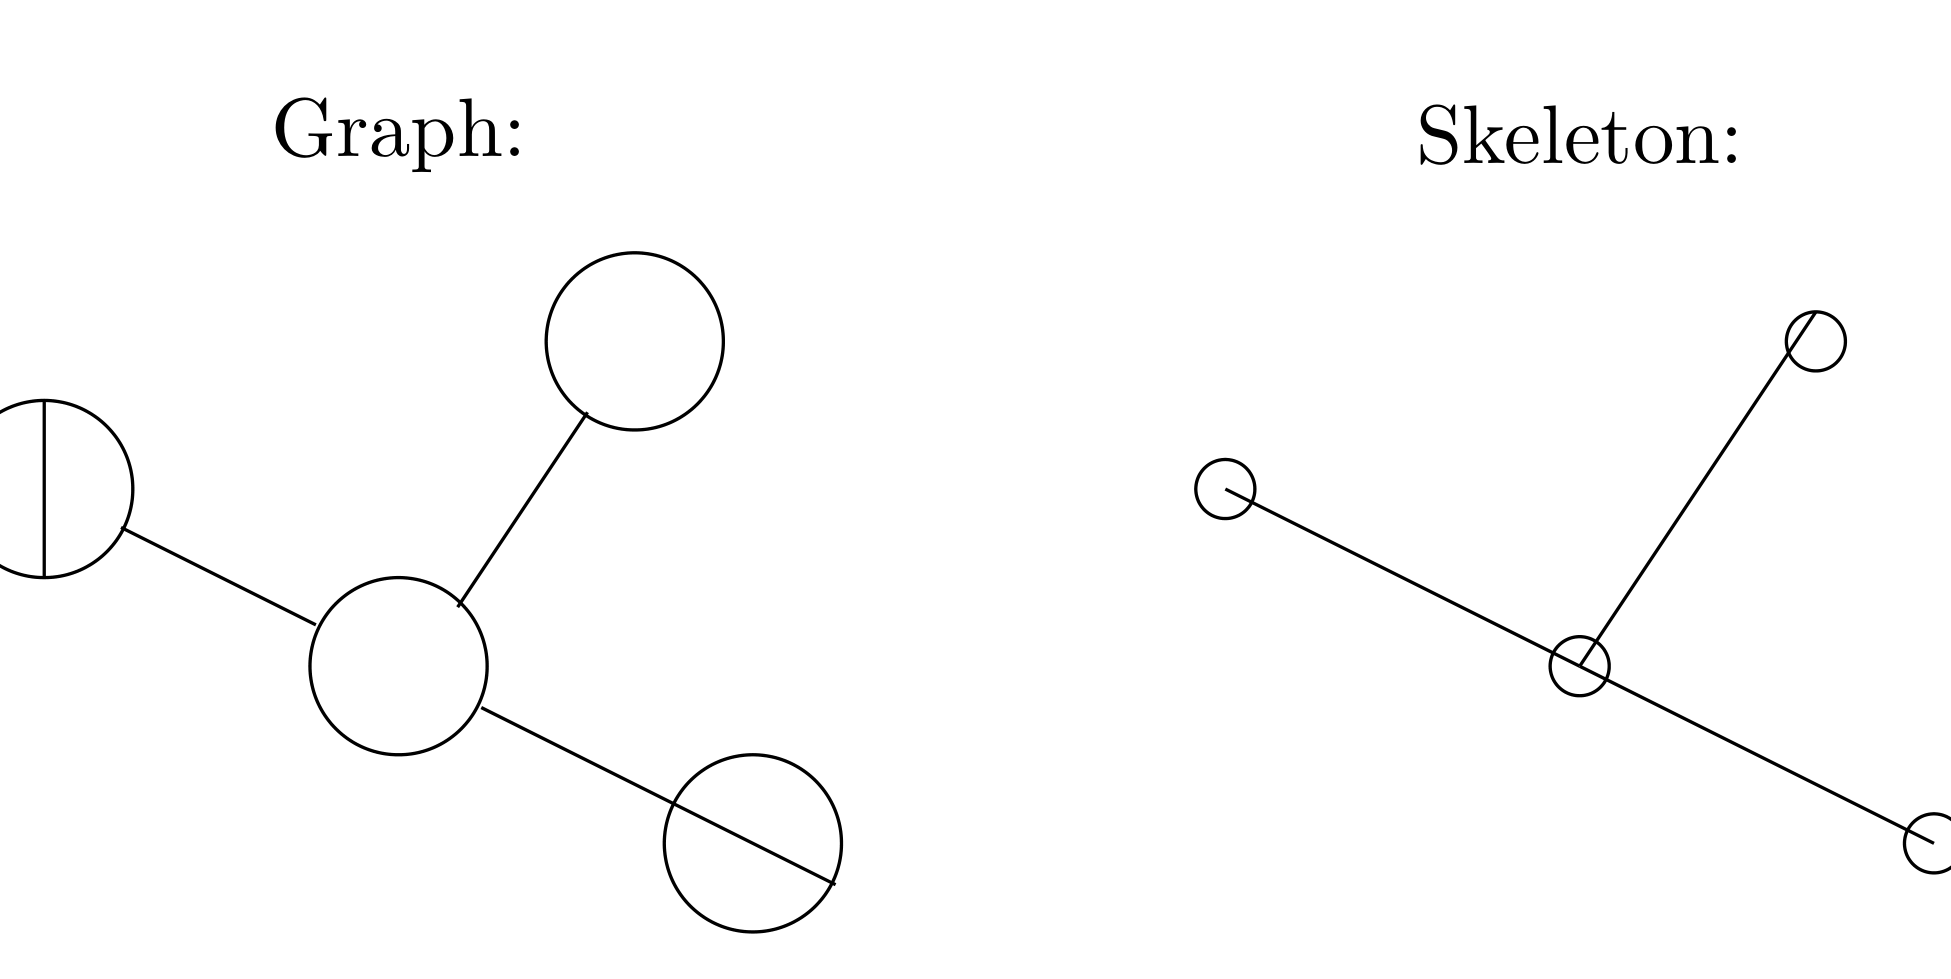
\includegraphics[width=8.26cm]{figures/fig-09.png}
  \caption{一个图的骨架。\figorig{49}{9}}
  \label{fig:9}
\end{figure}

容易看出引理 \ref{obv} 蕴含定理 \ref{effac}。事实上，它表明在 $\log\frac{Z_S}{Z_0}$ 的表达式中出现的所有连通图之和可以写成对骨架树的求和，于是每棵树的贡献（正比于）放在其顶点上的张量 ${\mathcal B}_i$ 的缩并，而 ${\mathcal B}_i$ 是所有带 $i$ 条外线的单粒子不可约图的振幅的（加权）和。
\end{proof}

\subsection{单粒子不可约图与 Legendre 变换}

回忆\emph{Legendre 变换}的概念。设 $f$ 是向量空间 $Y$ 上的光滑函数，使得由 $x\to df(x)$ 给出的映射 $Y\to Y^*$ 是微分同胚。则可如下定义 $f$ 的 Legendre 变换：对 $p\in Y^*$，设 $x_0=x_0(p)$ 是函数 $(p,x)-f(x)$ 的临界点（即方程 $df(x)=p$ 的唯一解），则 $f$ 的 Legendre 变换是由
$$
L(f)(p)=(p,x_0)-f(x_0).
$$
定义的 $Y^*$ 上的函数。容易看出 $L(f)$ 的微分也是微分同胚 $Y^*\to Y$（事实上是 $df(x)$ 的逆），且 $L^2(f)=f$。

\begin{example} 设 $f(x)=\frac{ax^2}{2}$，$a\ne 0$。则 $px-f=px-\frac{x^2}{2}$ 在 $p=\frac{x}{a}$ 处有临界点，临界值为 $\frac{p^2}{2a}$。于是 $L(\frac{ax^2}{2})=\frac{p^2}{2a}$。更一般地，若 $f(x)=\frac{B(x,x)}{2}$，其中 $B$ 是 $Y$ 上的非退化对称形式，则 $L(f)(p)=\frac{B^{-1}(p,p)}{2}$。例如，质量为 $m$ 的粒子其拉格朗日量 $\frac{mv^2}{2}-U(x)$ 关于速度 $v=\dot{x}$ 的 Legendre 变换就是它的哈密顿量（能量）$\frac{p^2}{2m}+U(x)$，反之亦然。事实上，这一点在完全一般的情形下都成立，这正是 Legendre 变换在经典力学与场论中起重要作用的原因。
\end{example}

注意，驻相公式表明 Legendre 变换是 Fourier 变换的经典类比。事实上，Feynman 密度 $e^{\frac{iS(x)}{\hbar}}dx$ 的（适当归一化的）Fourier 变换 $\hbar^{-\frac{d}{2}}\int_V e^{\frac{i(-(p,x)+S(x))}{\hbar}}dx$（其中积分按分布的意义理解）取对数后，当 $\hbar\to 0$ 时的渐近展开的首项为 $-\frac{iL(S)(p)}{\hbar}$。

现在我们在定理 \ref{Feyn} 的情形下考察定理 \ref{effac}。于是 $S(x)=\frac{B(x,x)}{2}+O(x^3)$，我们考察
$$
Z(p)=\hbar^{-\frac{d}{2}}\int_Ve^{\frac{(p,x)-S(x)}{\hbar}}dx.
$$
由定理 \ref{effac}，有
$$
\log\frac{Z(p)}{Z_0}=-\hbar^{-1}S_{\rm eff}(x_0,p),
$$
其中有效作用量 $S_{\rm eff}(x,p)$ 是对单粒子不可约图的求和，而 $x_0=x_0(p)$ 是它的临界点。

现在必须有 $S_{\rm eff}(x,p)=-p\cdot x+S_{\rm eff}(x)$，因为唯一含 1 价内顶点（对应于 $p$）的 1PI 图就是只有一条边的图：它把一个内顶点与一个外顶点相连（故给出项 $-p\cdot x$，而其他图不含 $p$ 顶点）。这表明 $\hbar\log\frac{Z(p)}{Z_0}$ 是 $p\cdot x-S_{\rm eff}(x)$ 的临界值。于是我们证明了以下结论。

\begin{proposition} 有
$$
S_{\rm eff}(x)=L(\hbar\log\tfrac{Z(p)}{Z_0}),\ \hbar\log\tfrac{Z(p)}{Z_0}=L(S_{\rm eff}(x)).
$$
\end{proposition}

物理学家将该结果表述如下：有效作用量是 $\hbar$ 乘以量子关联函数生成函数之对数的 Legendre 变换（反之亦然）。

\begin{exercise} 计算
$$
S(x)=\tfrac{x^2}{2}-g(x+\tfrac{x^3}{6}).
$$
的 $\log\frac{Z}{Z_0}$ 的一圈贡献。利用此结果，计算只含 1 价与 3 价顶点的、带 n 个顶点的带标号一圈图的数目（注意重边与自环！）。通过直接枚举顶点数较少的这类图来检验你的答案。
\end{exercise}

\begin{exercise}
求只含 1 价与 4 价顶点的带 n 个顶点的带标号树的数目 $a_n$ 的指数生成函数 $\sum_n a_n\frac{z^n}{n!}$。答案可以用多项式的反函数表示。
\end{exercise}

\begin{exercise} 求 $S(x)=\frac{x^2}{2}-\frac{gx^3}{6}$ 的有效作用量的一圈贡献。即，有 $S_{\rm eff}=S+\hbar S_1+O(\hbar^2)$，需要求出 $S_1$。需要考虑哪些 Feynman 图？
\end{exercise}

\begin{exercise} 考虑热方程 $u_t=\frac{1}{2}\Delta_B u$，其中 $\Delta_B$ 是第 \ref{inse} 小节中定义的附属于 $B$ 的 Laplace 算子。它由热流 $u(x,t)=e^{\frac{t\Delta_B}{2}}u(x,0)$ 解出。证明：作用量 $S(x)=\frac{B(x,x)}{2}-\widetilde S(x)$ 的有效作用量 $S_{\rm eff}$ 可以计算为作用量 $S^\circ(x):=\frac{B(x,x)}{2}-\widetilde S^\circ(x)$ 的无自环 1PI Feynman 图贡献之和，其中 $\widetilde S^\circ(x):=e^{\frac{\hbar\Delta_B}{2}}\widetilde S(x)$ 是用时间为 $\hbar$ 的热流变换 $\widetilde S$ 所得。
\end{exercise}

\bigskip
\noindent\rule{\textwidth}{0.6pt}
% [Tutor Note: 本章小结——§3.7–3.12 把“树”当作组合骨架：临界点方程的不动点迭代给出树展开，Cayley 定理与加权矩阵树定理是它在 d=1、完全图与着色情形下的特例；§3.13–3.14 把同一骨架提升到量子层面：把连通图按桥收缩成以 1PI 子图为顶点的骨架树，得到有效作用量的圈展开，其经典（树）部分恰为原作用量临界值取负。最易出错处有两点：一是 Legendre 变换的符号与变量——原文定义 L(f)(p)=(p,x_0)-f(x_0) 以 p 为自变量，故命题写成 S_eff(x)=L(ℏ log(Z/Z_0))；文献中常写成 Γ[φ]=sup_J(Jφ-W[J])，两者只差 W 的整体符号约定，务必沿途跟踪。二是 L²(f)=f 只在临界点唯一（凸性）时成立，多临界点处只能逐分支谈论，量子修正下更要小心。]
